\section{Durchführung}
\label{sec:Durchführung}

Bei diesem Versuch wir ein Röntgengerät, dargestellt in Abbildung 
\ref{fig:Aufbau}, verwendet. 

\begin{figure}
\centering
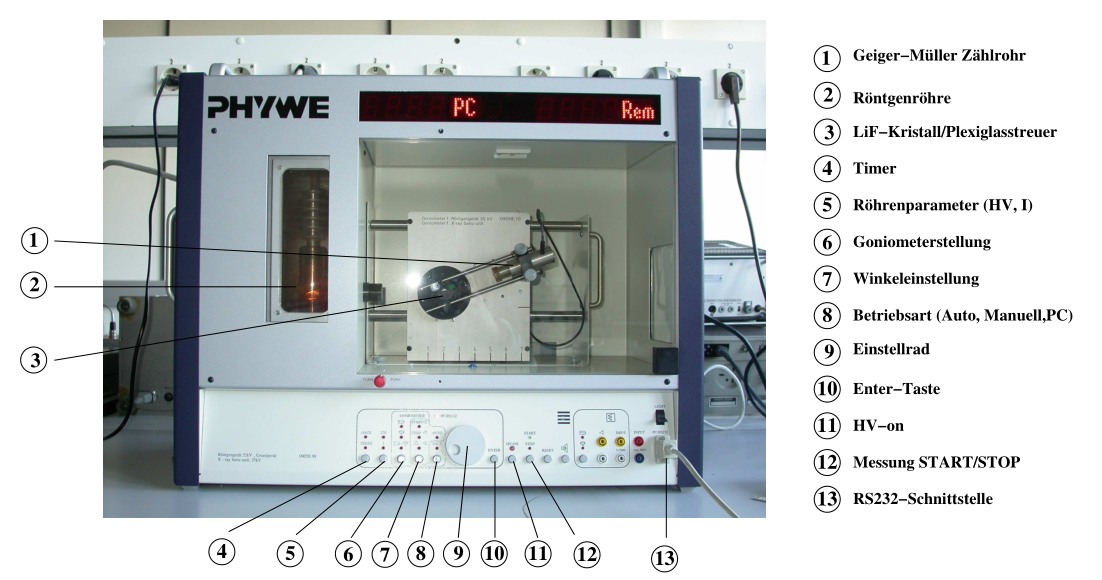
\includegraphics[scale=0.5]{content/aufbau1.png}
\caption{Röntgengerät. [1]}
\label{fig:Aufbau}
\end{figure}

Es besteht grunsätzlich aus einer Kupfer-Röntgen-Röhre, welche auf einen 
um sich selbst rotierbaren LiF-Kristall gerichtet ist. Auf einer Kreisbahn 
um den Kristall kann wiederrum ein auf jenen gerichtetes Geiger-Müller-Zählrohr
bewegt werden.